\chapter{Dataset}

\section{Sources}

\paragraph{}
We combined multiple dataset to create our voices' corpus:

\begin{itemize}
	\item 
	\textbf{Emo-DB} \cite{krautdb} 800 recording spoken by 10 actors (5 males and 5 females); 7 emotions: anger, neutral, fear, boredom, happiness, sadness, disgust
	
	\item
	\textbf{EMOVO} \cite{costantini-etal-2014-emovo} 6 actors who played 14 sentences; 6 emotions: disgust, fear, anger, joy, surprise, sadness
	
	\item 
	\textbf{Emov-DB} \cite{adigwe2018emotional} Recordings for 4 speakers- 2 males and 2 females; The emotional styles are neutral, sleepiness, anger, disgust and amused
	
	\item 
	\textbf{JL corpus} \cite{jl-corpus} 2400 recording of 240 sentences by 4 actors (2 males and 2 females); 5 primary emotions: angry, sad, neutral, happy, excited. 5 secondary emotions: anxious, apologetic, pensive, worried, enthusiastic
	
	\item 
	\textbf{Multimodal EmotionLines Dataset (MELD)} \cite{poria2019meld} has been created by enhancing and extending EmotionLines dataset. MELD contains the same dialogue instances available in EmotionLines, but it also encompasses audio and visual modality along with text. MELD has more than 1400 dialogues and 13000 utterances from Friends TV series. Each utterance in a dialogue has been labeled with— Anger, Disgust, Sadness, Joy, Neutral, Surprise and Fear
	
	\item
	The \textbf{Ryerson Audio-Visual Database of Emotional Speech and Song (RAVDESS)} \cite{livingstone_steven_r_2018_1188976} contains 7356 files (total size: 24.8 GB). The database contains 24 professional actors (12 female, 12 male), vocalizing two lexically-matched statements in a neutral North American accent. Speech includes calm, happy, sad, angry, fearful, surprise, and disgust expressions, and song contains calm, happy, sad, angry, and fearful emotions. We used only speeches
\end{itemize}

\section{Preprocessing}

\paragraph{Formats}
We were presented with a variety of audio formats, such as WAW and OGG, from those we created the MEL spectrograms with \texttt{librosa}'s help, a Python library to handle audio signals from heterogeneous sources

\paragraph{Spectrograms}
Each audio sample was loaded with a sampling rate of 44100 Hertz, file which had a different sampling rate were automatically resampled by the library; then each sample was divided, when possible, in multiple segments of 1.75 seconds of length each; finally spectrograms were computed and saved to single channel PNG file.

\paragraph{Classes}
Each PNG was saved in a sub-directory named after its class.

\paragraph{Multiprocessing}
Python's multiprocessing capabilities were used to speed-up the computation.

\paragraph{Procedure and example}
Here it follows the procedure used to generate the images:

\lstinputlisting[language=Python, linerange={20-89}]{../preprocess.py}

\begin{figure}[H]
	\centering
	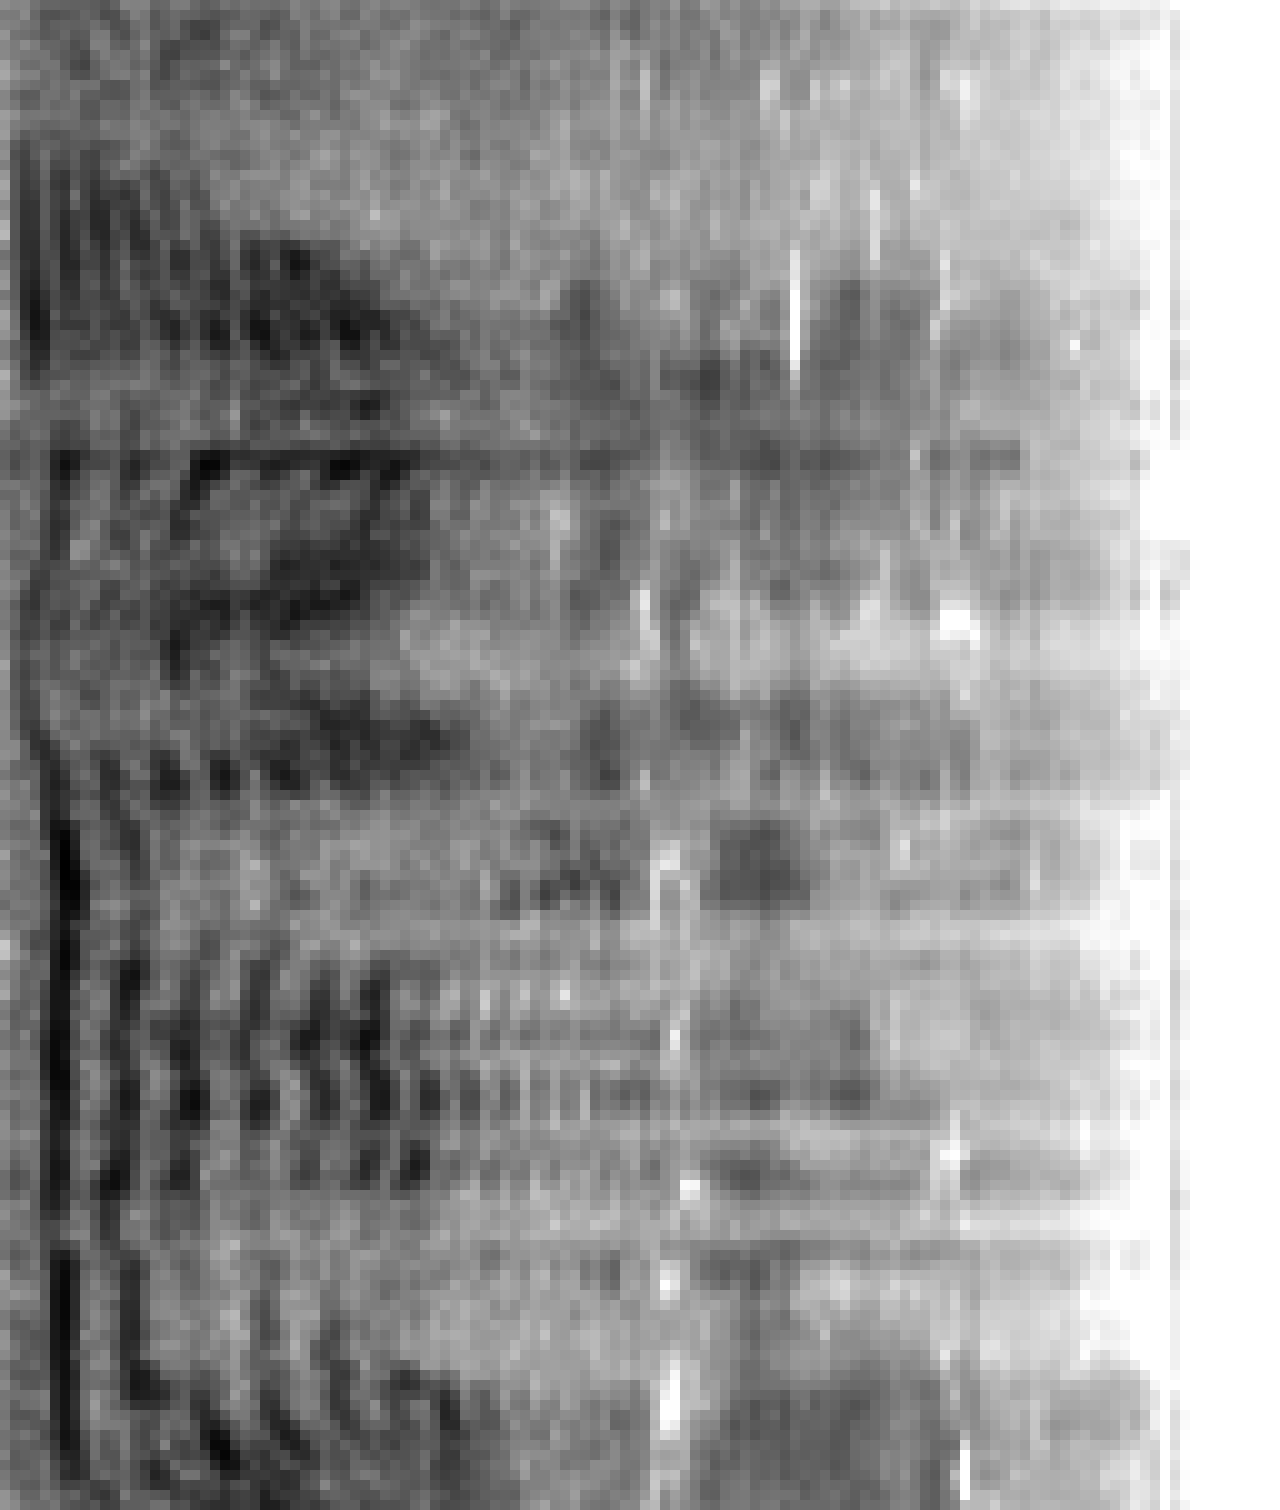
\includegraphics[width=0.7\linewidth, angle=90, interpolate=false]{assets/ex1.big.png}
	\caption{Example of spectrogram of length 1.75 seconds}
	\label{fig:ex2}
\end{figure}

\paragraph{Voice extraction}
We tried to isolate human voice from other background noise through librosa's buil-in methods but results were unsatisfactory as the accuracy and F1-score dropped significantly, thus we used the raw audios without any cleaning --- i.e. we set \texttt{ISOLATE\_VOICE = False} in the generation program.

It's certainly possible to improve models' performances with proper audio cleaning technique but we lack both the skill and the time to dive deeper into the manner. For example, we could have tried to cut frequencies that are not used by humans' voices.

\section{Classes}

\paragraph{}
We obtained the following dataset:

\vspace{10mm}
\begin{tabular}{|c|r|r|}
	\hline
	Class & Cardinality & Ratio \\
	\hline\hline
	SURPRISE	& 1063 & 9.51\% \\
	\hline
	SADNESS		& 1132 & 10.13\% \\
	\hline
	NEUTRAL		& 2811 & 25.15\%\\
	\hline
	HAPPINESS	& 2807 & 25.15\%\\
	\hline
	DISGUST		& 1204 & 10.77\%\\
	\hline
	ANGER		& 2160 & 19.33\%\\
	\hline\hline
	\textbf{Total} & 11177 & 100\% \\
	\hline
\end{tabular}

\paragraph{}
Pictures are 128x151 in size.

